\section{Status in Paderborn}

\subsection{"Städtische" Daten}
\begin{frame}[t]{Status in Paderborn}
 % add data source as url somewhere
 \begin{figure}
  \centering
  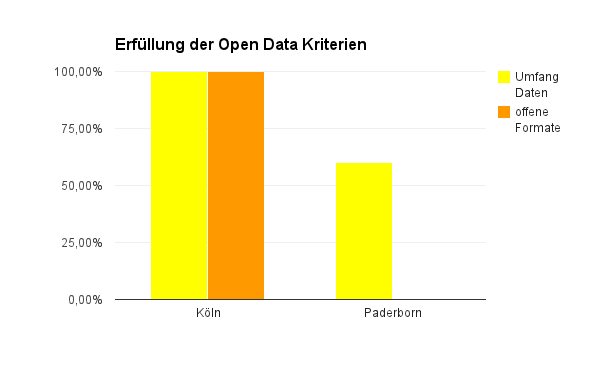
\includegraphics[scale=0.45]{section_paderborn_status.png}
 \end{figure}
 \begin{itemize}
  \item Paderborn \textbf{leicht} über Durchschnitt (49\%, 0,03\%)
  \item Keine Maschinenlesbaren Formate, aber relativ guter Datenumfang
 \end{itemize}
\end{frame}

\subsection{openstreetmap}
% add data source as url somewhere
\begin{frame}[t]{Status in Paderborn}
 \begin{figure}
  \centering
  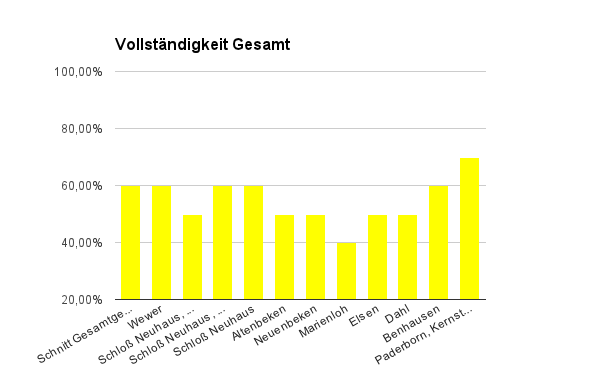
\includegraphics[scale=0.5]{section_paderborn_osm_overall.png}
 \end{figure}
\end{frame}

% add data source as url somewhere
\begin{frame}[t]{Status in Paderborn}
 \begin{figure}
  \centering
  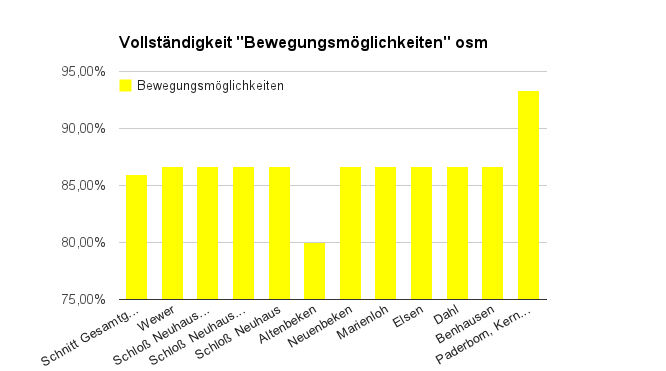
\includegraphics[scale=0.5]{section_paderborn_osm_move.png}
 \end{figure}
\end{frame}